\documentclass[titlepage]{article}
\usepackage[utf8]{inputenc}
\usepackage{graphicx,wrapfig}
\graphicspath{{images/}}
\usepackage{amsmath}
\usepackage{wrapfig}
\usepackage{subcaption}
\usepackage{array}
\usepackage{float}
\usepackage[export]{adjustbox}
\usepackage{setspace}
% ADDITION
\setlength{\parindent}{0pt}
% --------
\usepackage{geometry}
 \geometry{
 a4paper,
 total={170mm,257mm},
 left=20mm,
 top=20mm,
 }
\usepackage[utf8]{inputenc}
\usepackage[english]{babel}
\usepackage{fancyhdr}
 
% \pagestyle{myheadings}
% \markboth{lady4932}{Calibrating a digital camera for computer vision}
\pagestyle{fancy}
% \fancyhf{}
\fancyhead[LE,RO]{Nihaar Shah}
\fancyhead[RE,LO]{lady4932}
% \fancyfoot[CE,CO]{\leftmark}
% \fancyfoot[LE,RO]{\thepage}
 
% \renewcommand{\headrulewidth}{2pt}
% \renewcommand{\footrulewidth}{1pt}
\usepackage{listings}
\usepackage{color}

\definecolor{dkgreen}{rgb}{0,0.6,0}
\definecolor{gray}{rgb}{0.5,0.5,0.5}
\definecolor{mauve}{rgb}{0.58,0,0.82}

\lstset{frame=tb,
  language=Matlab,
  aboveskip=3mm,
  belowskip=3mm,
  showstringspaces=false,
  columns=flexible,
  basicstyle={\small\ttfamily},
  numbers=none,
  numberstyle=\tiny\color{gray},
  keywordstyle=\color{blue},
  commentstyle=\color{dkgreen},
  stringstyle=\color{mauve},
  breaklines=true,
  breakatwhitespace=true,
  tabsize=3
}
\begin{document}
\title{B1 report-Calibrating a digital camera for computer vision}
\author{Nihaar R. Shah}
\date{18 January 2016}

\maketitle
%Introduction to the document
\doublespacing
\section{Introduction}
Resectioning or calibrating a camera means to estimate the parameters of the lens and the sensor device of the camera. To estimate these parameters one needs 3D world coordinates and their \textit{corresponding} 2D image points using multiple images of a calibration pattern. Assuming there aren't any inaccuracies (due to noise or outliers) in these correspondences and the position of camera relative to object is known then we can simply apply equations to obtain the required parameters. \\
However, in reality there will always be errors in matching up the corresponding points of image distance between a projected point and a measured one. We can apply RanSac algorithm to reduce outliers by choosing the best fitting points only. Assuming the noise in the correspondences is mainly Gaussian, we can minimize the variance between image locations and predicted locations. This optimization is known as bundle–adjustment. Our project implements these two procedures to find a near accurate K-Matrix of required parameters.
% Aim and motivation subsections of Intro
\subsection{Aim}
The aim is to estimate and optimize the intrinsic parameters of a simplified ideal pinhole based model of a camera. My report attempts to \textit{test} and \textit{explain} the algorithms used and suggests further actions that can be taken to achieve a commercial solution.
\subsection{Motivation}
Knowledge of intrinsic parameters is very useful in finding real world distances of planar objects (from a single camera) if we know the position where the camera is mounted. Inversely, if we know distances in an image then we can estimate the camera location. Using stereo cameras we can estimate depth as well, which is useful in \textbf{visual odometry} which has many applications in robotics for example in localization for \textbf{self-driving cars}.
% %
% % The KMatrix equation 
% \begin{align} \label{KMatrix}
% K=
%   \begin{bmatrix}
%   \alpha f & \gamma f & t_u \\ 
%   0        & \beta f  & t_v \\ 
%   0        &    0     &  1 
%   \end{bmatrix}
% \end{align}
%Starting a new section
\section{Outline}
% Simulation subsection of Outline
\subsection{Simulation}
In practice we would use an actual calibration object like a checkerboard pattern with known distances between edges. In this project, we simulate the calibration pattern. We use a known K-matrix with pre-defined parameters to make correspondences.
In reality the K matrix is unknown. Through algorithms edge detection of the calibration object is possible. We then feed the known distances between these edges to the program to build the correspondences. In addition we input the 6 degrees of freedom needed to define the location of object in world coordinates (e.g. using lidar sensors). Instead, in this project we have functions to position the camera and position the object in world coordinates. A good test that these functions are working as expected is to view a simulated cube as seen by the camera as shown in figure (1). Note the 4 MegaPixel(MP) camera hence 2000 x 2000 pixel dimensions of the image. The cube was built by inputting each edge as a combination of cube vertices.
\begin{figure}
\begin{subfigure}{0.5\textwidth}
\includegraphics[width = 3.5cm,height = 3.5cm]{SimulateCube.eps}
\caption{Simulated cube in camera's field of vision.}
\label{wrap-fig:9}
\end{subfigure}
% Build noisy image figure
\begin{subfigure}{0.5\textwidth}
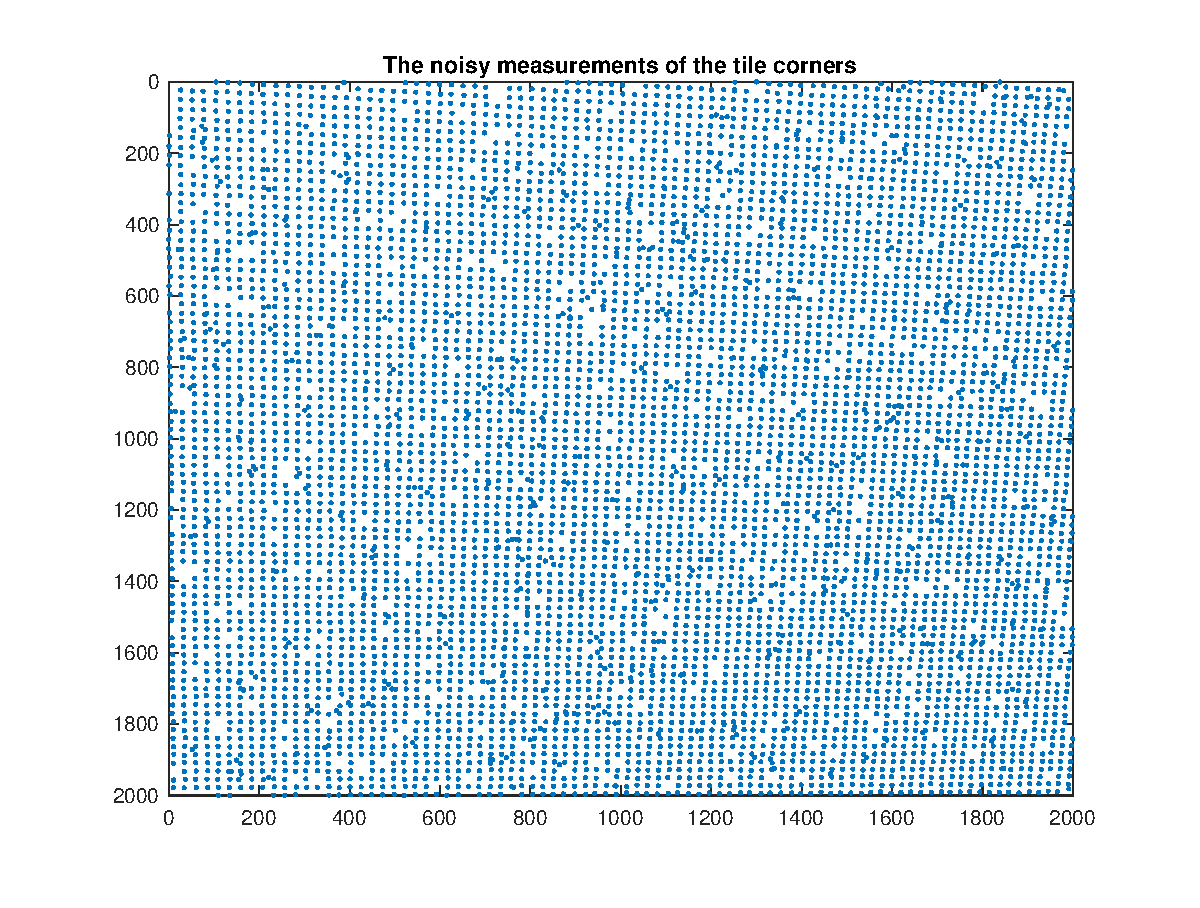
\includegraphics[width = 4.5cm,height = 4.5cm]{GridImage.eps}
\caption{Noisy grid image appears on camera sensor.}
\label{noisy-grid}
\end{subfigure}
\end{figure}
%
% Subsection on Estimation
\subsection{Initial Estimate}
\subsubsection{Estimating Homography}
% The object to image conversion equation 
% \begin{equation}\label{uv-to-xy}
% \begin{bmatrix}
%   U\\ 
%   V\\ 
%   S 
%   \end{bmatrix}
%         = \textbf{K}
%          \begin{bmatrix}
%  \textbf{r1} & \textbf{r2} & \textbf{t}
%          \end{bmatrix}
%         \begin{bmatrix}
%   x\\ 
%   y\\ 
%   1 
%   \end{bmatrix}    
%       =  \begin{bmatrix}
%   h_{11}  & h_{12} & h_{13} \\ 
%   h_{21}  & h_{22} & h_{23} \\ 
%   h_{3_1}  & h_{32} & h_{33} 
%   \end{bmatrix}
%           \begin{bmatrix}
%   x\\ 
%   y\\ 
%   1 
%   \end{bmatrix}    
%         \end{equation}
We build correspondences between object coordinates (xy) and image points (uv) using position of object relative to camera. \textbf{K} parameters and the positional parameters are packed in the Homography elements $h_{i,j}$ and our task is to estimate \textbf{H}.
%
% The object to image conversion equation 
% \begin{equation}
%     \label{Regressor}
%   \begin{bmatrix}
%   u\\ 
%   v
%   \end{bmatrix}
%         = 
%       \begin{bmatrix}
%  x & y & 1 & 0 & 0 & 0 & -ux & -uy \\
%  0 & 0 & 0 & x & y & 1 & -vx & -vy
%   \end{bmatrix}
%   \begin{bmatrix}
%   h_{11}\\ 
%     .\\
%     .\\
%   h_{32}
%   \end{bmatrix}
%  \implies \mathbf{p}_{j} = \mathbf{\phi}_{j}  \mathbf{h}_{j}
%       \end{equation}
Using j = 1 to 4 known point correspondences we can stack the 4 matrices to build a determinate system of equations having 8 unknowns and 8 equations. Solving this system will give us an estimate of Homography. But how do we know that the 4 points we have chosen to estimate it are all inliers? Thus we perform RanSac to select those pixel points which fit well with the \textbf{H}. Now we have an over-determined system with as many equations as the inliers. This system of equations is \textbf{P} =  \textbf{$\Phi$} \textbf{H}. We expect the correspondences to be noisy, hence no exact solution will exist. We therefore use \textbf{least squares minimization} as shown in Equation (3).
\begin{equation}
\label{Least Squares}
min |\mathbf{\Phi} \mathbf{H} - \mathbf{P}|^2 \implies \frac{\partial {|\mathbf{\Phi} \mathbf{H} - \mathbf{P}|^2}}{\partial\mathbf{(parameters)}} = 0 \implies \mathbf{H} = [\mathbf{\Phi}^T \mathbf{\Phi}]^{-1} \mathbf{\Phi} \mathbf{P}
\end{equation}
$\Phi$ (i.e. Regressor made of uv and xy coordinates) and \textbf{P} (i.e. uv coordinates) are \textit{known}. We use \textbf{singular value decomposition} (svd) to compute the inverse in Equation 5 because that is computationally cheaper than using matlab inverse (See Section 4.2). This is called pseudo-inverse. Now we have computed an estimate of the Homography.
\subsubsection{Estimating K-Matrix from Homography}
\label{estK}
Finally we want to estimate the K matrix from this Homography using 3 images of the grid taken from different angles. We pre-multiply both sides by K inverse. $\mathbf{H_j} = \lambda_j \mathbf{K_j} [\mathbf{r_1} \mathbf{r_2} \mathbf{t}]_j \implies \mathbf{K}^{-1} \mathbf{H_j} = \lambda_j [\mathbf{r_1} \mathbf{r_2} \mathbf{t}]_j$
% K from H equation
% \begin{equation}
%     \label{K from H}
%     \mathbf{H_j} = \lambda_j \mathbf{K_j} [\mathbf{r_1} \mathbf{r_2} \mathbf{t}]_j \implies \mathbf{K}^{-1} \mathbf{H_j} = \lambda_j [\mathbf{r_1} \mathbf{r_2} \mathbf{t}]_j
%     \end{equation}
We use the orthogonal property of the rotation matrix by pre-multiplying the Homography with the rotation matrix transpose (or inverse) $\mathbf{H_j}^T (\mathbf{K_j^{-1}})^{T} \mathbf{K_j}^{-1} \mathbf{H_j} = \lambda^2 \mathbf{I}$. 
    % \begin{equation}
    %   \label{inverse-transpose}
    %     \mathbf{H_j}^T (\mathbf{K_j^{-1}})^{T} \mathbf{K_j}^{-1} \mathbf{H_j} = \lambda^2 \mathbf{I}
    % \end{equation}
This equation holds true for each image j and can be used to make a homogeneous equation of form Ax=0 to solve for $\mathbf{\phi} = \mathbf{({K}^{-1})^T} \mathbf{K}^{-1}$ again using $svd(\mathbf{A}) = \mathbf{U} \mathbf{D} \mathbf{V}^T$ and right singular vector of matrix $\mathbf{\phi}$ associated with the \textit{smallest} singular value. This is because for a homogeneous system any vector $\mathbf{x}$ in the null space of \textbf{A} is a solution hence any column of $\mathbf{V}$ whose corresponding singular value is zero is a solution. If we want a particular solution then we might want to pick the solution $\mathbf{x}$ with the smallest length $|\mathbf{x}|^2$. We then obtain \textbf{K} from $\Phi$ using \textit{cholesky factorization} because we note that $(\mathbf{K}^{-1})^T$ is an upper triangular matrix and $K^{-1}$ a lower triangular matrix.
% Starting subsection called Optimization
\subsection{Optimization}
So far we have reduced outlier effects using RanSac. Gaussian noise still prevails. We can tackle this using optimization of the cost-function (\textbf{E}) defined as the least squares error between estimated and true values of uv. $\mathbf{E} =\frac{1}{2} \Sigma(Estimated [u'v'] - True [u v])^2$
Note that least squares form of cost function is an efficient way to eliminate noise but not outliers as it heavily penalizes Outliers. Thus, we have chosen the two step approach - RanSac followed by least squares optimization. This is a convex optimization problem (cost function is quadratic) hence we expect the global and local minimum to be the same. We decompose the Homography into the K-Matrix and positional parameters and then use this to predict the positions of points in the image using these transformation matrices and the current best camera matrix. The square of this minus the actual positions serves as our convex cost function.\\
We will use the \textbf{Levenberg-Marquardt algorithm} to adjust parameters and decide when the minimum is reached. Steepest descent is a method to reach minimum by varying parameters $\delta$ \textbf{p} along the steepest \textit{downhill} direction on the surface i.e. pointing along the \textit{negative} gradient vector. $\delta \mathbf{p} = -(\frac{\partial \mathbf{E}}{\partial\mathbf{p}})^T = \mathbf{g_n}$.
% Gradient descent equation
% \begin{equation}
% \label{steepest_descent}
% \delta \textbf{p} = -(\frac{\partial \mathbf{E}}{\partial\mathbf{p}})^T = g_n
% \end{equation}
%  
Newton steps method is based on taking the derivative of Taylor's expansion in N-dimensions as shown in Equation \ref{Newton_Step}   
% Newton step equation 
\begin{equation}
  \label{Newton_Step}
  \nabla (f(\textbf{x}+\delta\textbf{x}))=0 \implies \mathbf{g_n} + \mathbf{H_n} \delta p = 0\\
  \implies \delta{\mathbf{p}}=-\mathbf{H_n}^{-1}\mathbf{g_n}
\end{equation}
This gives the iterative update $\mathbf{x_{n+1}}=\mathbf{x_n}-\mathbf{H_n}^{-1} \mathbf{g}_n$ where $\mathbf{H_n}$ is the Hessian matrix $\frac{\partial^2 \mathbf{E}}{\partial \mathbf{p}^2}$. It is better to perform line search which ensures global convergence hence we introduce the parameter $\mu$ in Equation \ref{Newton_Gradient}
% Newtonstep-Gradient descent  equation 
\begin{equation}
\label{Newton_Gradient}
\mathbf{x_{n+1}}=\mathbf{x_n}-\mu\mathbf{H_n}^{-1} \mathbf{g}_n   
\text{ And combining Equations \ref{Newton_Step} and \ref{Newton_Gradient} } (\mathbf{H_n}+\mu\mathbf{I})\delta \mathbf{p}= -\mathbf{g}_n
\end{equation}
% \begin{equation}
%   \label{Final_Newton_Gradient}
%   (\mathbf{H_n}+\mu\mathbf{I})\delta \mathbf{p}= -\mathbf{g}_n
% \end{equation}
By solving for $\delta\mathbf{p}$ we we know the vector along which to change our parameters for the next iteration. We re-compute the cost at the new parameters and assess whether to reject the parameters or accept them as well as whether to increase or decrease $\mu$ i.e. we can control between Newton steps and gradient descent.
%-------------------------------------------------------------------------------------------------------
% Start section on the overview of structure
\section{Overview of the Structure}
\subsection{Data Structure}
When designing code you have to consider how to encapsulate the data so that flows are clear and match the control structure. I stuck to follow a structure of many interacting functions instead of creating large objects with many tasks. For e.g. in the Jacobian function I used Rodrigues function to make Rotation matrix from angle-axis instead of doing that calculation inside the Jacobian function (shown later).
Another e.g. in Jacobian function is I made a function for the task of perturbation because: less scope of error and \textbf{re-usability}. This modular structure also is compiler efficient and useful to scale up. Someone using this code for calibration may not input valid parameters so I validate parameters before running a function but there's a risk of passing parameters in the wrong order. Thus structures are good for passing long lists of parameters as the named fields are safer. Cell structure was used for storing data as the objects stored had unknown and variable sizes.
\subsection{Control Path}
\begin{center}
\textbf{FlowCharts for Algorithms used}\\
\end{center}
\begin{figure}[H]
\begin{subfigure}{0.5\textwidth}
   \includegraphics[width = 7cm,height = 18cm]{Ransac_flowchart.png}
   \caption{Estimation task involving RanSac}
   \label{Ransac_Flow}
\end{subfigure} 
\begin{subfigure}{0.5\textwidth}
    \includegraphics[width = 7cm,height = 18cm]{optim-flowchart.png}
    \caption{Optimization:the L-M algorithm}
  \label{Optim_Flow}
\end{subfigure} 
\caption{Flow charts for the two algorithms used to reduce Outliers and Noise respectively.}
\end{figure}
\textbf{RanSac flow}\\
RanSac algorithm eliminates outlier points - in this case pixels displaced from their true positions in the calibration image. While estimating homography from the edges of the checkerboard we take 4 random point correspondences to build our regressor $\Phi$. To ensure these points are a true representation of the objects (inliers) we perform RanSac.
%
We use RanSac to choose only \textit{that} homography estimate which best agrees with maximum number of points on the checkerboard. The flowchart in Figure \ref{Ransac_Flow} shows this algorithm.
Note that UV cordintes are the known points or true points. We multiply the estimated homography with the xy object coordinates to obtain estimated U’V’. RanSac compares the difference between the U’V’ estimated via homography and the true UV with a threshold MaxError and populates a vector BestConsensus that satisfies this threshold as acceptable inliers. 
We construct our Regressor of the over-constrained system and use svd to find the least squares estimate of our final homography if the condition number is “good” as accurate inverse is possible. As good coding practice I catch error using 'try' 'catch' to ensure inverse exists. With a good homography estimate it is straightforward to compute K using svd as mentioned in Section \ref{estK}.\\
\textbf{Optimization flow}\\
The algorithm controls the search to move from steepest descent to newton steps depending on how well the last search performed. 
The feedback mechanism is that if error has increased after changing the parameters along a certain direction then the weighting $\mu$ is increased reducing the step-size and causing the algorithm to just search downhill. If the error has reduced then we are \textit{closer} to the minimum so we search in the neighborhood itself using Newton steps.
% \begin{center}
% \textbf{FlowCharts for Algorithms used}\\
% \end{center}
% \begin{figure}[H]
% \begin{subfigure}{0.5\textwidth}
%   \includegraphics[width = 7cm,height = 18cm]{Ransac_flowchart.png}
%   \caption{Estimation task involving RanSac}
%   \label{Ransac_Flow}
% \end{subfigure} 
% \begin{subfigure}{0.5\textwidth}
%     \includegraphics[width = 7cm,height = 18cm]{optim-flowchart.png}
%     \caption{Optimization:the L-M algorithm}
%   \label{Optim_Flow}
% \end{subfigure} 
% \caption{Flow charts for the two algorithms used to reduce Outliers and Noise respectively.}
% \end{figure}
% \subsection{Why our approach?}
% \begin{figure}[H]
% \begin{subfigure}{0.5\textwidth}
% \includegraphics[width = 4cm,height=4cm]{outlier.png}
% \caption{Outliers}
% \label{Ransac_Flow}
% \end{subfigure} 
% \begin{subfigure}{0.5\textwidth}
% \includegraphics[width = 4cm,height = 4cm]{noise.png}
% \caption{Noise}
% \label{Optim_Flow}
% \end{subfigure} 
% \caption{Graphical representation of impact of Least Squares minimization on Noise and Outliers.}
% \end{figure}
\subsection{Why our approach?}
\begin{figure}[H]
\begin{subfigure}{0.5\textwidth}
\includegraphics[width = 3.5cm,height=3.5cm]{outlier.png}
\caption{Outliers}
\label{Ransac_Flow}
\end{subfigure} 
\begin{subfigure}{0.5\textwidth}
\includegraphics[width = 3.5cm,height = 3.5cm]{noise.png}
\caption{Noise}
\label{Optim_Flow}
\end{subfigure} 
\caption{Graphical representation of impact of Least Squares minimization on Noise and Outliers.}
\end{figure}
Suppose you fit a straight line to data containing outliers, the usual method of least squares estimation is flawed. It will penalize outliers excessively and lead to poor fit. Thus we must first get rid of these outlier and \textbf{then} apply Least Squares optimization. This is precisely our method.

%-------------------------------------------------------------------------------------------------------
\section{Detailed Considerations}
\subsection{How to measure accuracy}
\label{Accuracy}
%
% screenshot of correspond variable data structure
\begin{figure}[H]
\begin{subfigure}{0.5\textwidth}
\label{Correspond}
\captionsetup{width=6cm}
\includegraphics[width = 6cm,height = 2.0cm]{Correspond_workspace.png}
\caption{No. of columns = all points on the grid}
\end{subfigure}
% screenshot of consensus data structure
\begin{subfigure}{0.5\textwidth}
\label{Consensus}
\captionsetup{width=6cm}
\includegraphics[width = 6cm,height = 2.0cm]{BestConsensus_workspace.png}
\caption{Contains all points on the grid}
\end{subfigure}
%\caption{Workspace data structures showing Correspondences and Consensus matrices}
\caption{The workspace data structure dimensions verify all points are inliers.}
\end{figure}
\textbf{\underline{Noise and Outlier Test}}\\
The simplest was to set the noise $\sigma$ and $\mu$ = 0 and pOutliers=0 in the Correspondence matrix.\\
\textbf{Hypothesis}: There are now \textit{only} inliers i.e. all correspondences are accurate so estimating homography from any 4 points should give error of $\approx$ 0, since u’=u and v’=v. \textit{No} points are excluded from Consensus vector. \\
\textbf{Result}: This was verified as seen in Figures 4 (a) and (b). Also K estimated is the same as the K-Matrix.\\
% 2nd experiment
\textbf{\underline{RanSac runs Test}}\\
The second experiment was to vary number of RanSac runs and examine its effects on the accuracy of $K_{estimated}$. The accuracy metric used was the $L_{1}$ norm because $p > 2$ norm penalizes greater deviations too much while p=0 or p=inf norm maybe less representative of all elements. A better metric may be $\%$ error but 4 of 5 elements of K are 0 hence it is hard to find $\%$ change from 0. The noise and pOutlier were control parameters.\\
\textbf{Hypothesis}: More RanSac runs means more number of homographies to choose from to use as best fit for correspondence points. Better outlier rejection, hence a more accurate K estimate.  \\
\textbf{Result}: The general trend corroborates this expectation as seen in Figure \ref{RansacRunsVsAccuracy}.
\begin{figure}[H]
% Plot of ransac vs accuracy
\begin{subfigure}{0.25\textwidth}
\includegraphics[width = 4.5cm, height=5cm]{HomogErrorVsRansacRuns.eps}
\caption{Number of RanSac runs.}
\label{RansacRunsVsAccuracy}
\end{subfigure}
% Plot of MaxError vs accuracy
\begin{subfigure}{0.25\textwidth}
\includegraphics[width = 4.5cm, height=5cm]{MaxErrorVsHomogError.eps}
\caption{MaxError in RanSac.}
\label{MaxErrorVsAccuracy}
\end{subfigure} 
\begin{subfigure}{0.25\textwidth}
\includegraphics[width = 8cm, height=4cm]{underfitting-overfitting.png}
\caption{Fitting}
\label{Fit}
\end{subfigure} 
\caption{Varying Ransac runs and MaxError to find effect on Accuracy.}
\end{figure}
\textbf{\underline{MaxError Test}}\\
% 2nd experiment of Maxerror vs accuracy
\textbf{Hypothesis}: Decreasing the MaxError means we are decreasing the threshold of accuracy (more strict) for an estimated u'v' to be part of consensus set. So we will have more strictly selected inliers discarding even slight deviations hence more accuracy.\\
\textbf{Result}: For both very high or very low MaxError values the accuracy drops. For very high MaxError there are too many points including many outliers so lowered accuracy in Fig. 5b . Why lower accuracy for low MaxError then? Because of \textbf{over-fitting} i.e. having too many parameters relative to the number of observations so estimate can overreact to minor fluctuations in the training data. If the max error is too low, there will be very few points (very selectively chosen) in the consensus and in the regressor for the robust inverse (svd) calculation. I wrote extra script to output how many points are there in Bestconsensus set for a given Max Error value and found that for MaxError of $10^{-4}$ and a noise $\sigma$ of 0.1 we just have 10 elements and this reduces if MaxError is further reduced or if noise $\sigma$ is increased. Homography has 9 parameters.
% ADDITION
\bigskip

% --------
% \vspace{2mm} 
\textbf{\underline{Test for Jacobian calculation}} \\
For optimization I calculate the jacobian matrix by writing \textit{forward-difference} function. The perturbation was set to 0.001 $\%$ of the parameter and we used a for-loop to manually differentiate (perturb, subtract and divide) with respect to each parameter and construct our blocks as shown in the code below:\singlespacing
 % insert code
\begin{lstlisting}
 % We are estimating the derivative using f'(x)=[f(x+dx)-f(x)]/dx w.r.t each of 11 parameters
% Perturb each K parameter by a small percent of itself turn by turn and store each perturbed matrix
k1 = KMatrix;
k1(1,1) = KMatrix(1,1)*perturbation; % ... and so on until k5(2,3)=KMatrix(2,3)*perturbation;
    
% Find new estimated uv from each perturbed kmatrix. This is f(x+dx) in f'(x)=[f(x+dx)-f(x)]/dx
fk1 = k1 * P *[XY; 1]; % ... and so on until fk5 = k5 * P *[XY; 1];
    
% This is f'(x). We divide by fk(3) to scale it back to original.
dk1 = (fk1(1:2)/fk1(3)-UVest)/(KMatrix(1,1)*(perturbation-1)); % ... and so on until dk5;
    
% Finally constructing our K parameters block consisting of 5 columns and 2*no. of points rows 
NKMATJACOB(2*a-1:2*a,:) = [ dk1 dk2 dk3 dk4 dk5 ];
\end{lstlisting}
To \textbf{test the accuracy} of this function, I wrote another function using \textbf{symbolic MATLAB toolbox} which textit{analytically} finds the \textit{entire} Jacobian and then I select the required blocks from that, as shown (some lines omitted for conciseness):
% insert more code
\begin{lstlisting}
% Parameters come from KMatrix, Rotation axis and Translation vector
K = sym('k',[3,3]);
RotAxis = sym('rot',[1,3]); % etc. for other parameters

% fin is calculated symbolically in terms of the 6 extrinsic parameters in P and 5 intrinisic in K
for i = 1:n
    XY = Correspond(3:4,BestConsensus(i));
    f = K * P * [XY' 1]';
    f = f/f(3);
    fin = [fin;f(1:2,1)];
end
Var = [(1,1),K(1,2),K(1,3),K(2,2),K(2,3),RotAxis(1,1),RotAxis(1,2),RotAxis(1,3),t(1,1),t(2,1),t(3,1)];
% symbolically forming the two blocks using the jacobian library function
JKMat = jacobian(fin,Var(1,1:5)); JFram = jacobian(fin,Var(1,6:11));

% Substituting in the parameters one by one like shown for K parameter below
J1 = subs(JKMat,K,KMatrixValues);
\end{lstlisting}
%
\doublespacing
MATLAB's 'jacobian' library function uses \textbf{symmetric central difference} and other algorithms. It's an analytic approach and more accurate than simply forward difference. However, it's computationally expensive as the zero-terms of the Jacobian are computed which can otherwise be avoided by only calculating the required blocks (as done in the former above). Both results were nonetheless similar, thus we prefer the first method.
%
\subsection{Is this simulation a good model of the real world?}
\label{realistic}
There are approximations and assumptions in any model. Here are a few: \\\textbf{\underline{A) I.I.D. Noise}} Principal sources of Gaussian noise in digital images arise during acquisition e.g. sensor noise caused by poor illumination, high temperature, transmission e.g. electronic circuit noise. A typical model of image noise is Gaussian, additive, independent at each pixel. Obviously, there are other noise sources that are \textit{not Gaussian} e.g. Salt-and-pepper noise (caused by analog-to-digital converter errors), Shot noise (statistical quantum fluctuations), Quantization noise (quantizing the pixels of a sensed image to a number of discrete levels), Anisotropic noise (noise sources show up with a significant orientation) etc. Thus Gaussian noise is an \textit{approximation} not totally representative of truth. Based on this assumption we have chosen cost function as a least squares minimization. \\\textbf{\underline{ B) Outliers}} An outlier in an image is often a region that has been occluded, an object that suddenly appears in one of the images, or a region that undergoes an unexpected motion (due to slight camera motion). Outlier modelling is a field on its own. We have used a \textit{simplistic} way of adding outliers at random pixels. \textbf{\underline{C) Lens distortion}} We have used an ideal pinhole simplification \textit{excluding} radial and tangential distortion. Radial Distrortion occurs when light rays bend more near the edges of a lens than they do at its optical center. The smaller the lens, the greater the distortion. Tangential distortion occurs when the lens and the image plane are not parallel.\\ \textbf{\underline{D) Algebraic approximations}}: For mathematical and computational simplicity we have used certain approximations. For instance to calculate matrix inverse we use svd \textit{'pseudo inverse'}. For determining stopping criterion, instead of comparing Gradient to 0 we set the criterion to a \textit{really low number} such as 1e-5. For computing the \textit{Hessian} as second partial derivatives we approximate it as $J^{T}J$ thus using the jacobian already calculated.
\section{Measures of Code Performance}
\subsection{Noise}
\begin{wrapfigure}{r}{5.5cm}
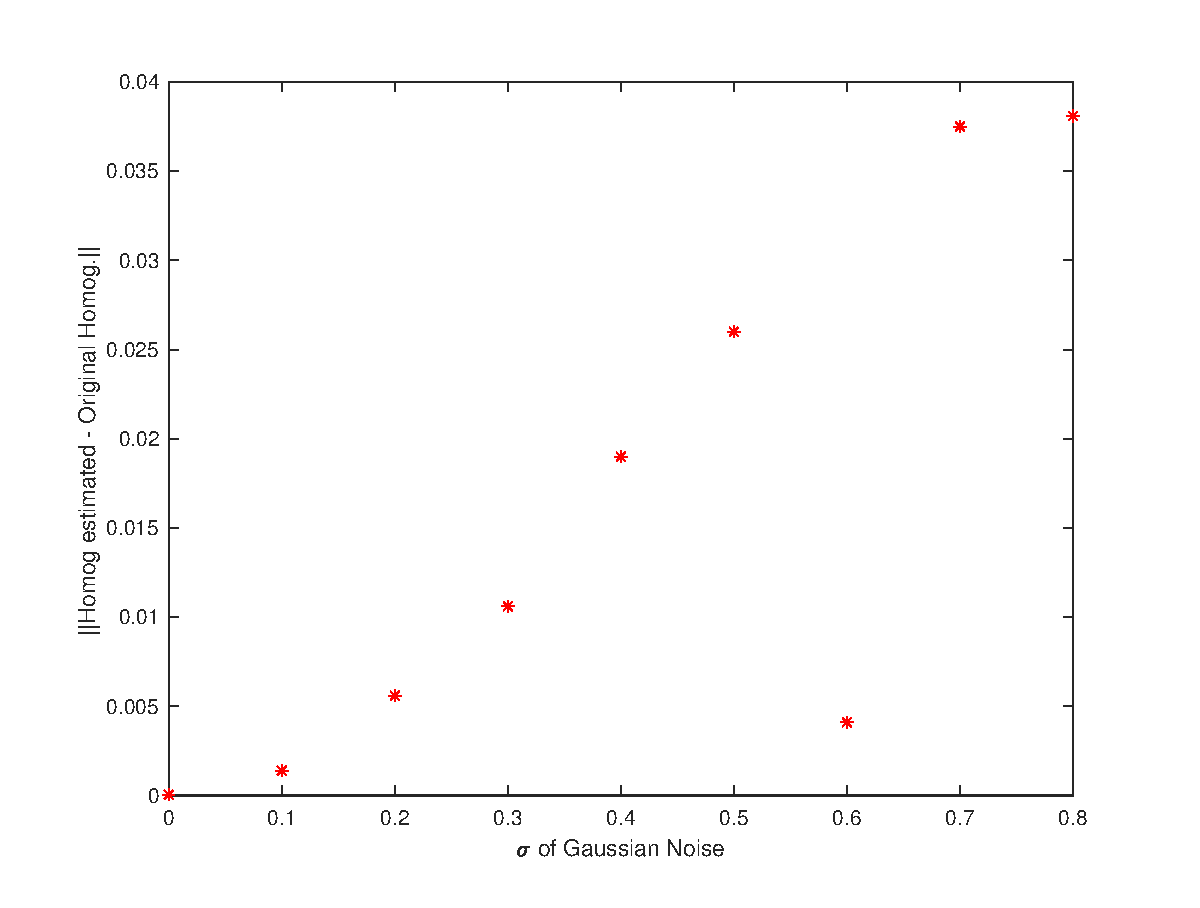
\includegraphics[width = 5.5cm, height=5.5cm]{HomogerrorVsNoiseVariance.eps}
\caption{Effect of varying noise variance on accuracy of estimation.}
\end{wrapfigure} 
Fig. 6 shows the trend that more the noise variance i.e. the image pixels of calibration image are more apart from their true values then the worse the error between the norm between true Homography matrix and the estimated. Although there is one outlier in the above trend, that is reasonable since we are randomly choosing points each time we run the estimate. So even with the same value of standard deviation and every other parameter, there will be variations in the error values which is why we can explain that as long as the trend is towards worse error with increased variance we can ignore this particular outlier.
\subsection{Speed}
% screenshot of correspond variable data structure
\begin{figure}[H]
\begin{subfigure}{0.5\textwidth}
\label{Correspond}
\includegraphics[width = 8.0cm,height = 3.5cm]{JacobianSym_timing.png}
\caption{Using library jacobian function.}
\end{subfigure}
% screenshot of consensus data structure
\begin{subfigure}{0.5\textwidth}
\label{Consensus}
\includegraphics[width = 8.0cm,height = 3.5cm]{singleImageJacob_timing.png}
\caption{Using forward difference.}
\end{subfigure}
%\caption{Workspace data structures showing Correspondences and Consensus matrices}
\caption{Timing performance for the two methods to compute Jacobian.}
\end{figure}
The Figure 7 shows how the analytic jacobian compares with the forward difference method. The self-time (i.e. the time taken in that particular function excluding the 'child' functions) for finding the Jacobian compares so:
\begin{verbatim}
% improvement = 0.068/(0.264-0.068) = 35 %
\end{verbatim}
While the total time taken i.e. includes the cumulative time over all the iterations and Ransac runs is incomparable 0.497s vs 108.64s. For calibration speed is less important than robustness but the two methods are almost equally accurate. Thus, we clearly prefer the approximate forward difference method. 
\section{Conclusions}
\subsection{How would I input real data?}
This project simulated the calibration image. In reality we would use an image of an actual calibration image and after calibration only deal with real images.The image would be treated as a matrix of intensities. Using edge detection we can find boundaries of objects within image \textbf{by detecting discontinuities} in brightness. Common algorithms include Sobel, Canny, Prewitt, Roberts, and fuzzy logic methods. The MATLAB command:
\begin{verbatim}
BW = edge(I,<type of algorithm>,threshold,direction)
\end{verbatim}
returns a binary image BW containing 1s where the function finds edges in the input image I and 0s elsewhere. It returns edges that are stronger than threshold. The input image I is an intensity or a binary image. Then we can enter known distances between them in the calibration image. After it is calibrated, we can use K-Matrix and Extrinisic parameters (from the position where we mount camera with respect to object) to find the real-world distances simply from an image of the planar objects. 
\subsection{How well did you do?}
\begin{figure}[H]
\begin{subfigure}{0.3\textwidth}
\includegraphics[width = 4.0cm,height = 2.5cm,left]{KAct.png}
\caption{Actual or true KMatrix.}
\end{subfigure}
\begin{subfigure}{0.3\textwidth}
\includegraphics[width = 4.0cm,height = 2.5cm,center]{kestim.png}
\caption{Estimated (cut off exp(3))}
\end{subfigure}
% screenshot of consensus data structure
\begin{subfigure}{0.3\textwidth}
\includegraphics[width = 4.0cm,height = 2.5cm,right]{opt-kmat.png}
\caption{Optim. K ($\approx$ estimated)}
\end{subfigure}
\caption{Comparing the final K-optimized and K-Estimated. Noise $\sigma$ =0.2, Stopping criterion value =1e-8 }
\end{figure}
Optimization performance of both methods is compared below by varying the Stopping Criterion (S.C.).
\singlespacing
% Insert table with different stopping criterions and the respective error norm
\begin{center}
\begin{tabular}{ | m{3cm} | m{2cm}| m{2cm} | m{2cm} | m{4cm} | } 
\hline
\textbf{Method} & \textbf{S.C.=1} & \textbf{S.C. = 1e-3} & \textbf{S.C.= 1e-8} & \textbf{S.C. = 1e-9} \\ 
\hline
Forward Difference & 42.0531 & 28.137 & 3.0238  & too many iterations \\ 
\hline
Analytical & 41.432 & 27.438 & 2.983 & too many iterations \\ 
\hline
\end{tabular}
\end{center}
\doublespacing
Accuracy metric used was $L_1$ norm as discussed in Section 4.1 although other metrics are also valid. Results from both methods were similar so I concluded that forward difference approximation might suffice in this case. It nevertheless served as a good test to verify Jacobian. To compare the two methods I kept noise $\sigma$ as an important control variable because the it has a direct impact on the optimization's performance.\\
The stopping criterion is chosen such that we can be reasonably sure that the minimum of the function has been reached i.e. the norm(gradient) is $\approx$ 0. Clearly keeping a high stopping threshold such as SC = 1 (see table) leads to lower accuracy. At the same time a very low SC = $10^{-9}$ meant the code never exited the optimization loop even after 100 iterations.
\subsection{Commercial product}
Finally, how close are we to make this into a commercial software? This has partly been answered in Section \ref{realistic} where we have discussed the assumptions, approximations and simplifications of this model. A commercial standard product may be able to improve on some of those for instance take the lens distortion into account or apply statistical noise and outlier models depending on the kind of image taken. Adding a GUI that can let the user input an image and automatically output the K-Matrix or the real-world distances from an image, are required for good user experience. The code performs reasonably well in speed, however, if more computational power is needed then the commercial solution should be able to harness GP-GPUs remotely if needed. For instance this could be a web-application which utilizes immense computational hardware in a data center. Lastly, there is a possibility to apply statistical testing to predict with a certain confidence level how accurate is our estimate.
\section{References}\singlespacing
1) Prof. Zisserman's and Prof. Daniel's slides on optimization\\
2) Noise: Jun Ohta (2008). Smart CMOS Image Sensors and Applications. CRC Press. ISBN 0-8493-3681-3.\\
3) Distortion:https://uk.mathworks.com/help/vision/ug/camera-calibration.html

\end{document}
